\section{算法对比分析（如有，与常用量子算法或经典算法在性能、精度、资源消耗等方面的对比）}
与纯经典 fixed 基线相比，本文方法在保持 LETKF 主骨架稳定性的前提下，实现了更低的 test\_1 误差；与 corr 这类直接结构化加权方案相比，本文避免了强接入带来的明显退化。与常见“量子调参”思路相比，本文量子模块不只做外层搜索，而是直接参与局地相似度建模，因此更贴近“量子增强同化机制”本身\cite{felix2024reservoir}. 与 Kotsuki 等人的量子退火数据同化相比，本文不把 4D-Var 整体转化为量子优化问题，而是仅在 LETKF 的局地结构层引入量子信息\cite{kotsuki2024qda}；与物理驱动局部化工作相比，本文不是利用流场物理特征重设局部化函数，而是利用量子相似度重设局地观测加权\cite{sarp2025localization}。

从资源消耗上看，当前方法每次只需构造 $4$ qubits 局地特征映射电路，线路规模小、计算代价可控，适合在受限量子模拟环境下复现。其代价低于大规模全局量子化方案，也更符合赛题实际约束。

为了更清楚地体现本文方法与现有思路的差异，这里将对比分析拆成四个层面。第一层是与经典强基线的对比，回答“量子增强是否真的有额外价值”；第二层是与 corr 等结构化权重方法的对比，回答“为什么不是任何结构化加权都有效”；第三层是与物理驱动局部化或经验局地化修正路线的对比，回答“为什么本文选择量子相似度而不是纯物理特征”；第四层是与常见量子调参式思路或量子退火 DA 路线的对比，回答“量子模块究竟是在外层搜索、整体替代，还是在内层参与同化机制”。只有把这几个问题分开说明，才能体现本文方法的独特位置。

\begin{figure}[htbp]
\centering
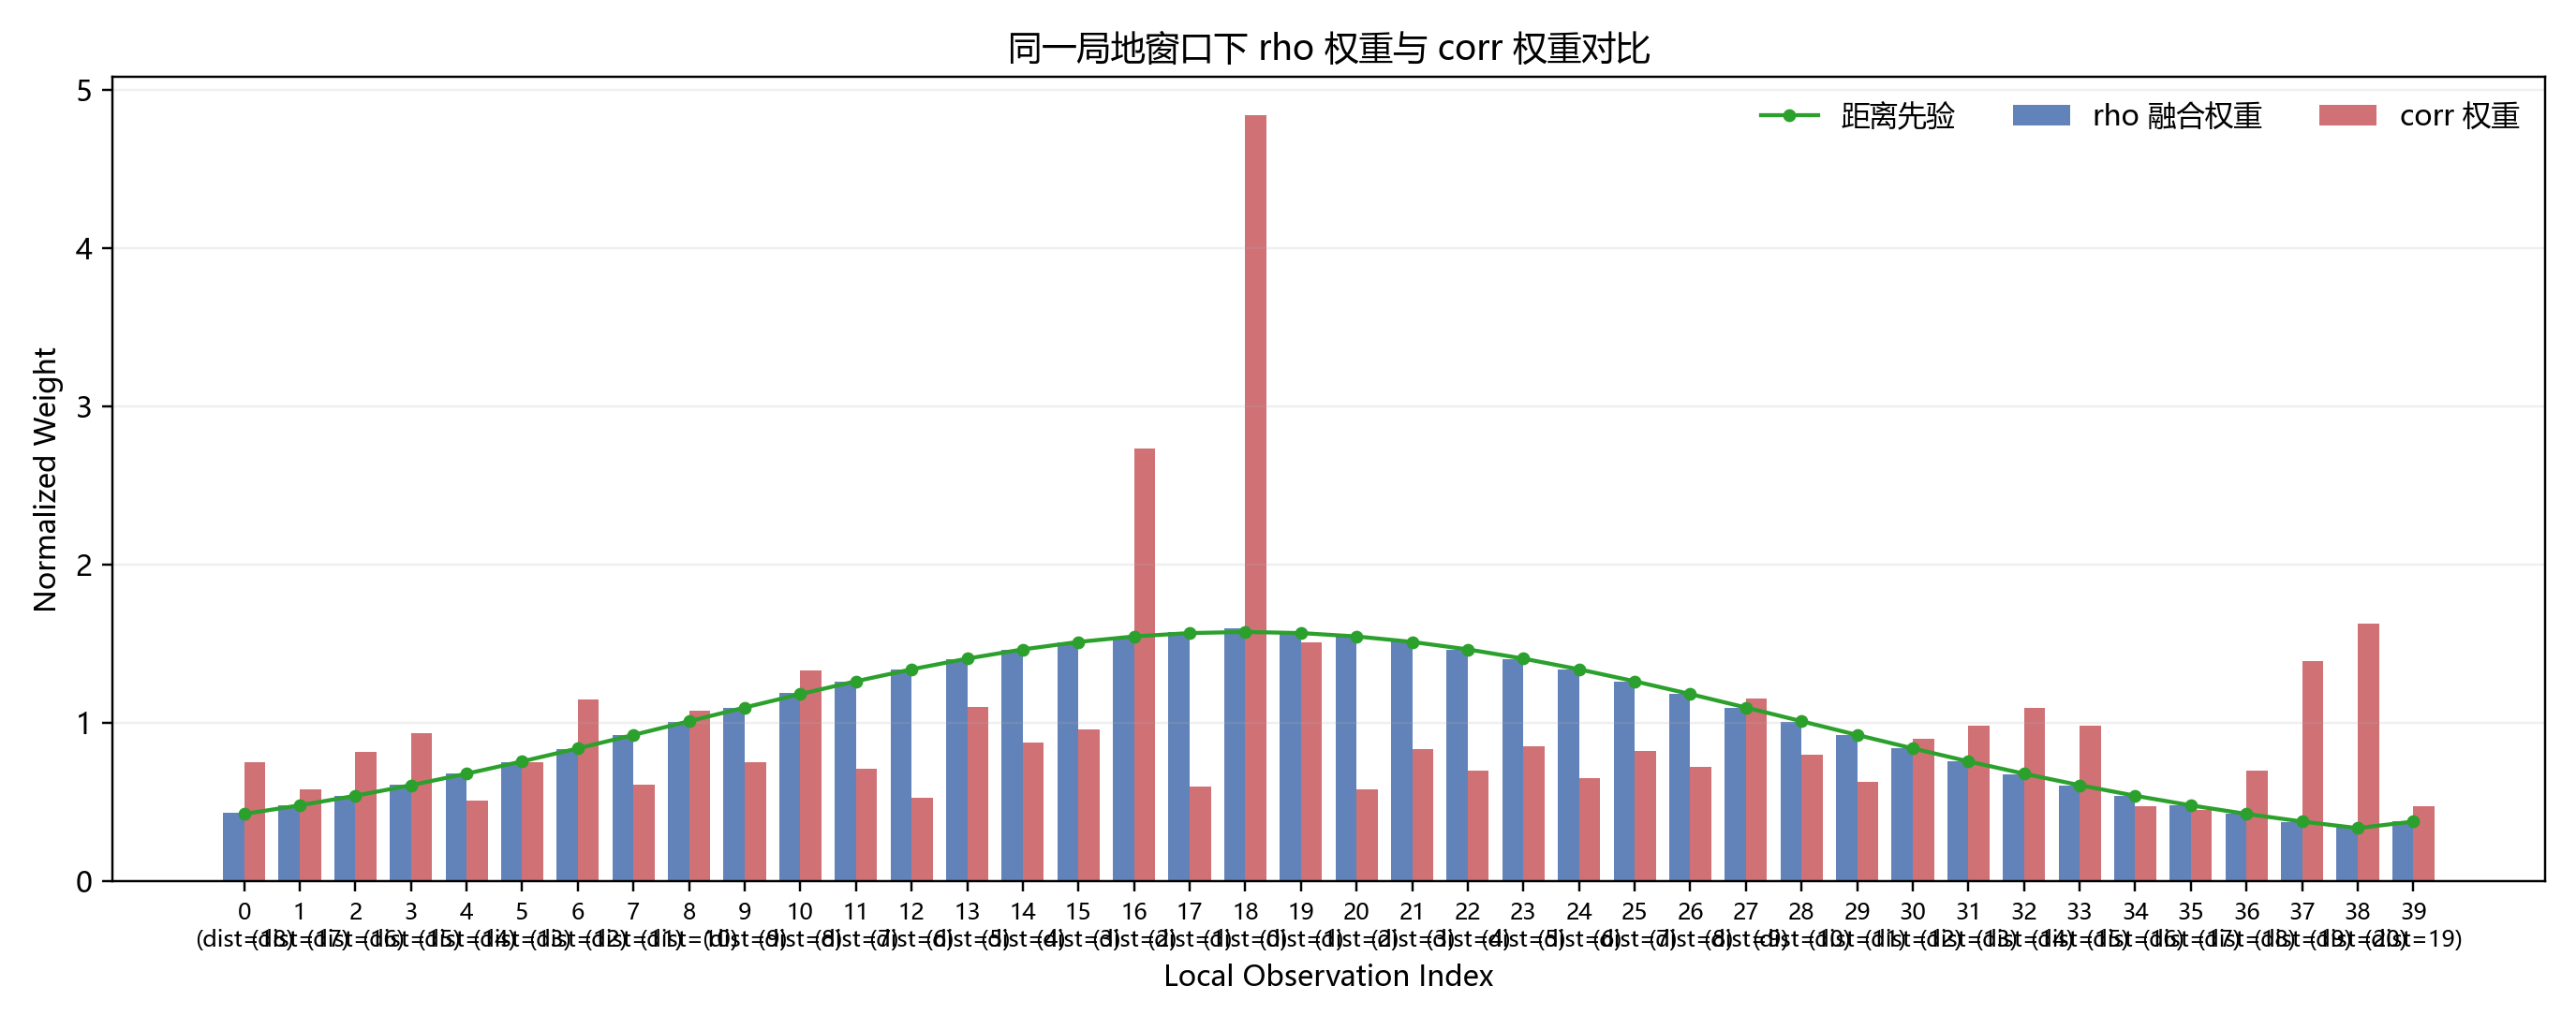
\includegraphics[width=0.92\linewidth]{figures/exp37_rho_vs_corr_weights.png}
\caption{同一局地窗口下，量子弱融合权重与 corr 权重的对比。}
\label{fig:weights}
\end{figure}

图 \ref{fig:weights} 进一步说明，本文方法与 corr 加权的差异不只是数值更优，而是机制不同。corr 权重更容易受局部相关性波动影响，而量子弱融合权重保留了距离先验，并用量子相似度做温和调制，因此整体更稳健。

换句话说，corr 更像是一种“单层直接加权”，而本文方法是一种“先保留经典局地结构，再叠加量子弱修正”的双层机制。这种差异决定了两者在稳定性上的表现不同：前者更容易因为局部相关性过强而退化，后者则更容易维持在可控的弱调制区间内。从数值上看，\texttt{corr} 的 test\_1 RMSE 为 $0.14279$，不仅没有优于 \texttt{fixed} 的 $0.12873$，反而恶化约 $10.93\%$；相比之下，最优量子弱融合配置为 $0.12698$，说明“结构化信息存在”并不自动意味着“任何结构化加权都有效”，关键仍在于结构信息如何进入经典更新。

\begin{figure}[htbp]
\centering
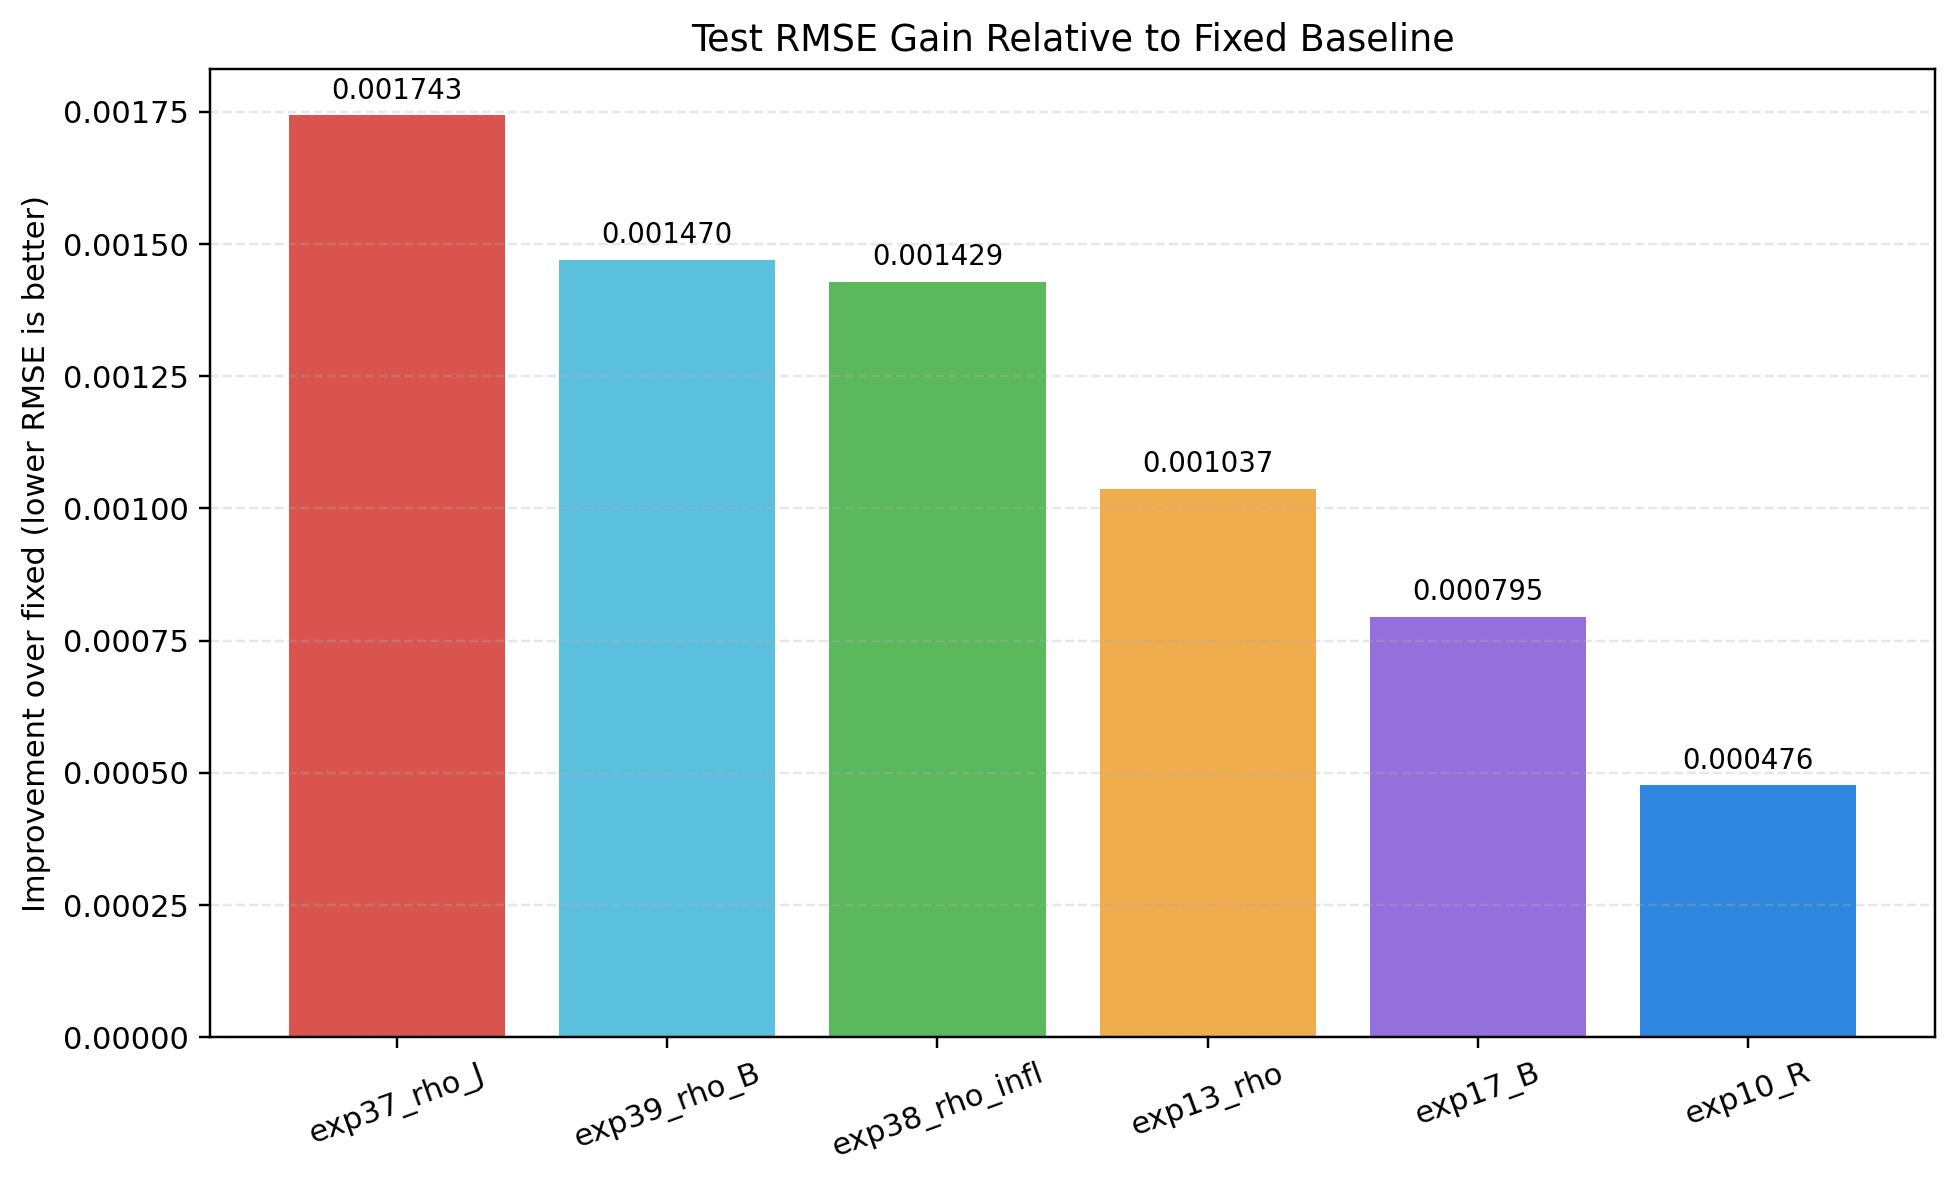
\includegraphics[width=0.92\linewidth]{figures/rmse_gain_over_fixed.png}
\caption{各候选高分方法相对 fixed 基线的 test\_1 RMSE 改善幅度。}
\label{fig:gain}
\end{figure}

图 \ref{fig:gain} 从更全局的候选方法角度补充了这一结论。该图展示了不同候选相对 fixed 的提升幅度，可以看到，在当前 exp37 全部六组受控配置里，四组量子弱融合都实现了正向改进，其中最优配置提升约 $1.35\%$，最弱配置也仍有约 $0.99\%$ 的提升。这说明本文的收益并非来自偶然挑中一个参数组合，而是来自对量子接入方式的有效筛选。

\begin{figure}[htbp]
\centering
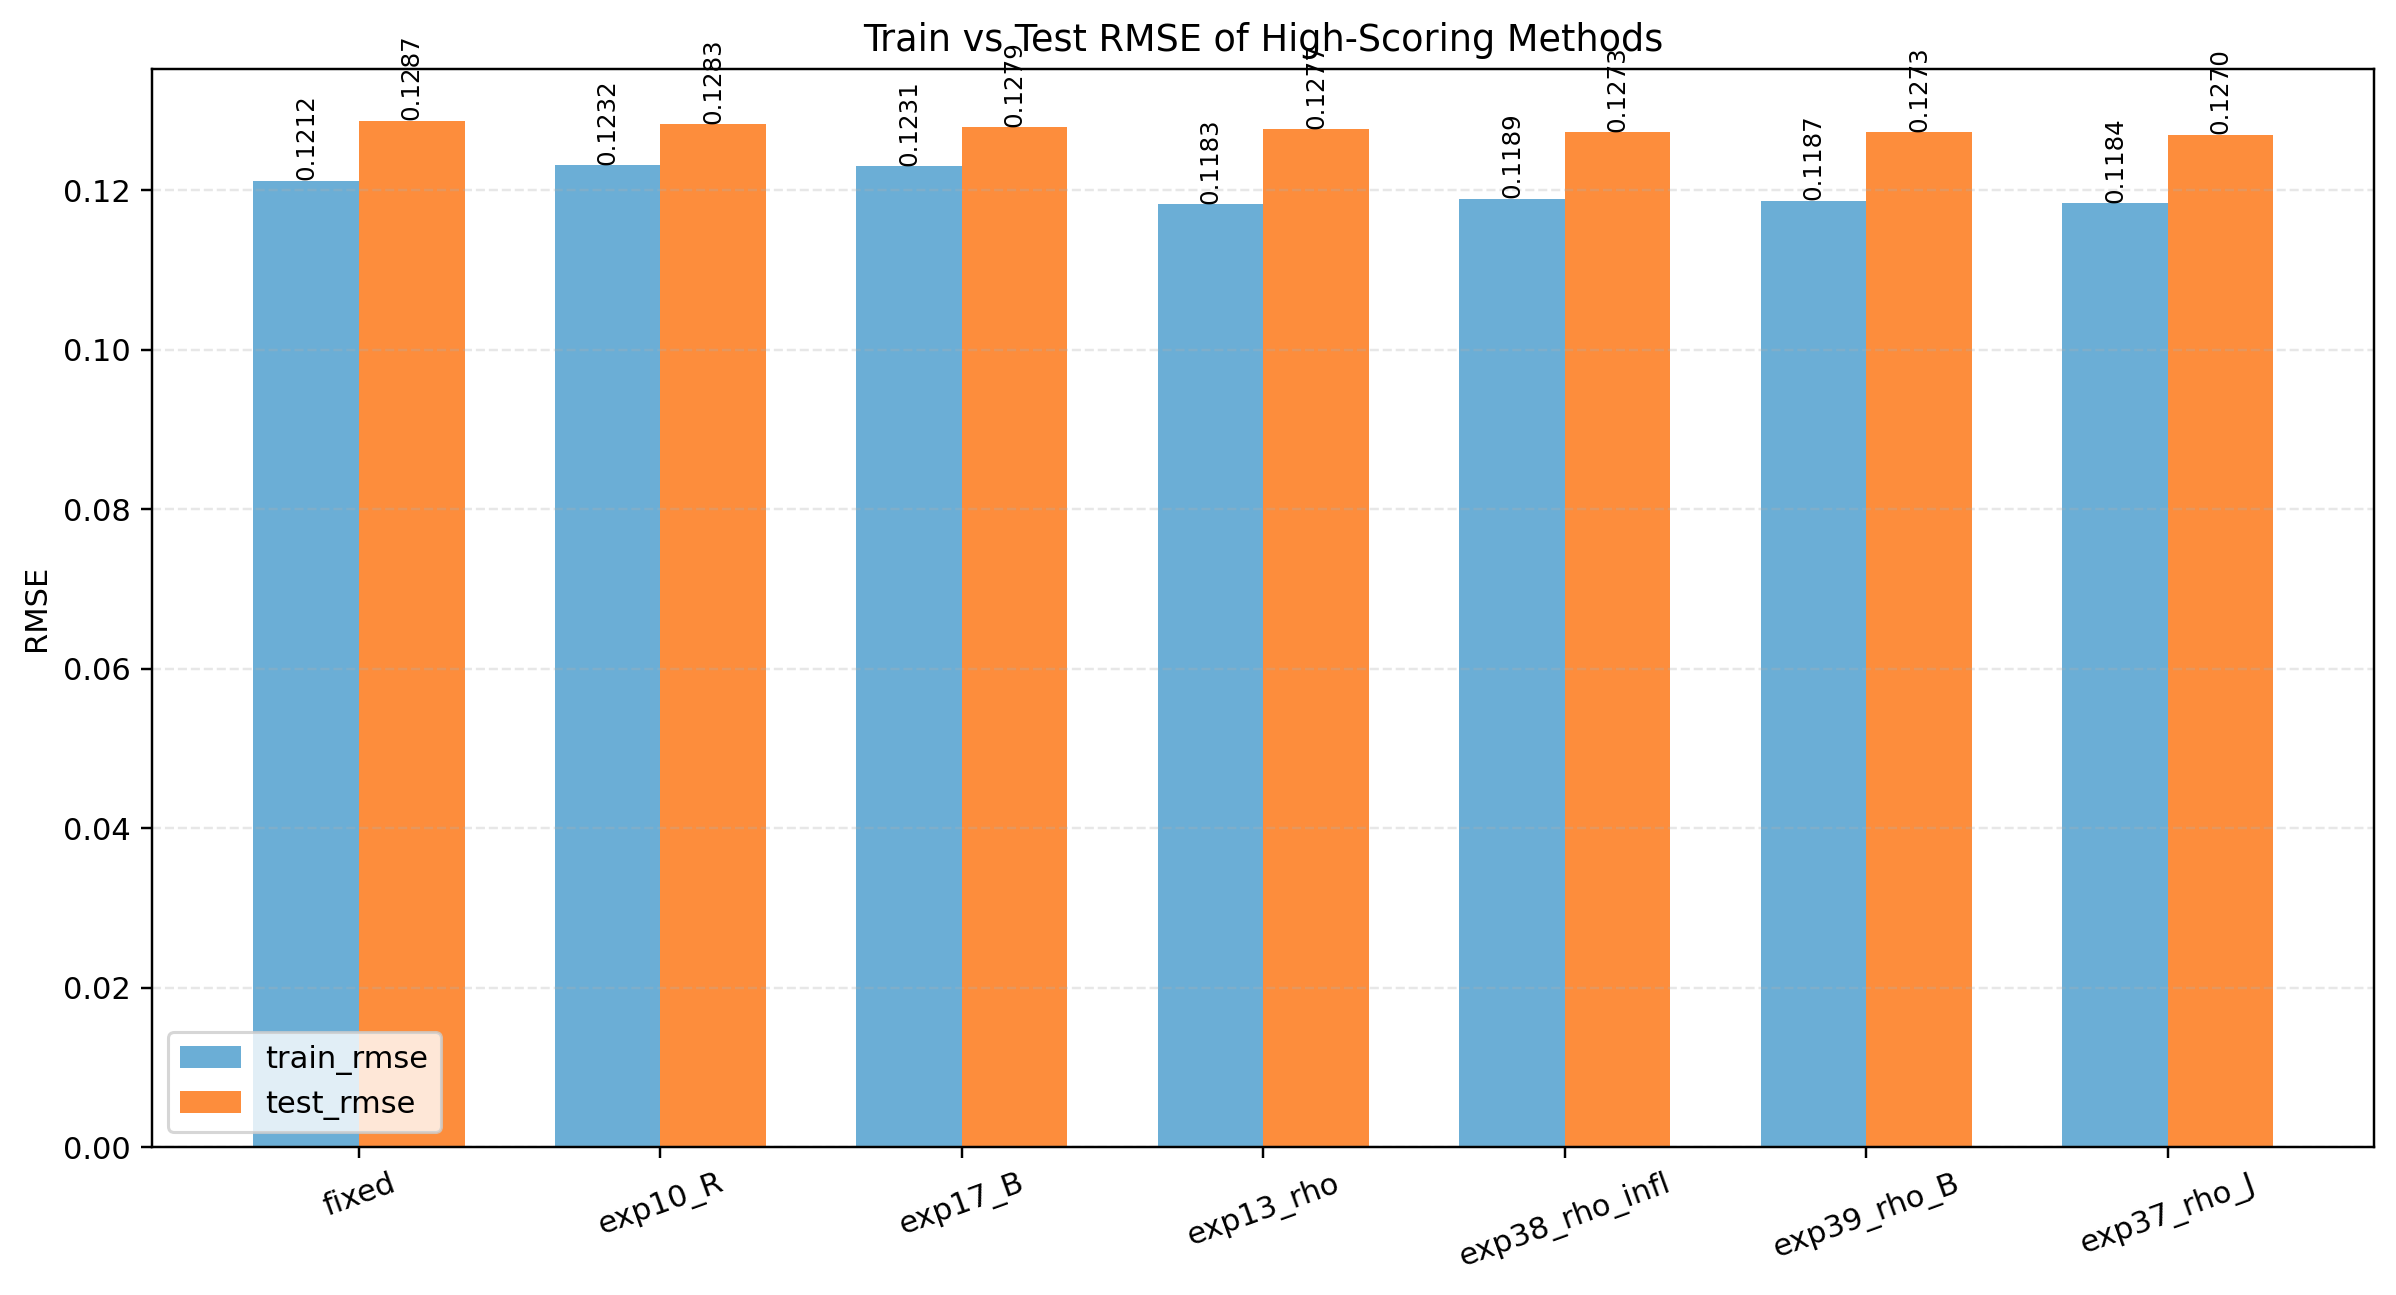
\includegraphics[width=0.92\linewidth]{figures/train_test_rmse_grouped.png}
\caption{高分候选方法在 train/test 上的 RMSE 分组对比。}
\label{fig:grouped}
\end{figure}

图 \ref{fig:grouped} 进一步说明，本文方法的优势并不只是训练端或局部测试端的偶然下降，而是在 train/test 两端都维持了较一致的表现。具体而言，最优量子弱融合配置的 train RMSE 为 $0.11844$，低于 fixed 的 $0.12120$；test\_1 RMSE 为 $0.12698$，同样低于 fixed 的 $0.12873$。对数据同化问题而言，这一点尤其重要，因为如果一个方法只在训练端改进明显、测试端退化，则说明它只是把局部结构拟合得更激进，而不具备真正的泛化能力。当前主线方案在这张图中的位置，更接近一种“稳健增益”而非“高风险高波动”方案。

\begin{figure}[htbp]
\centering
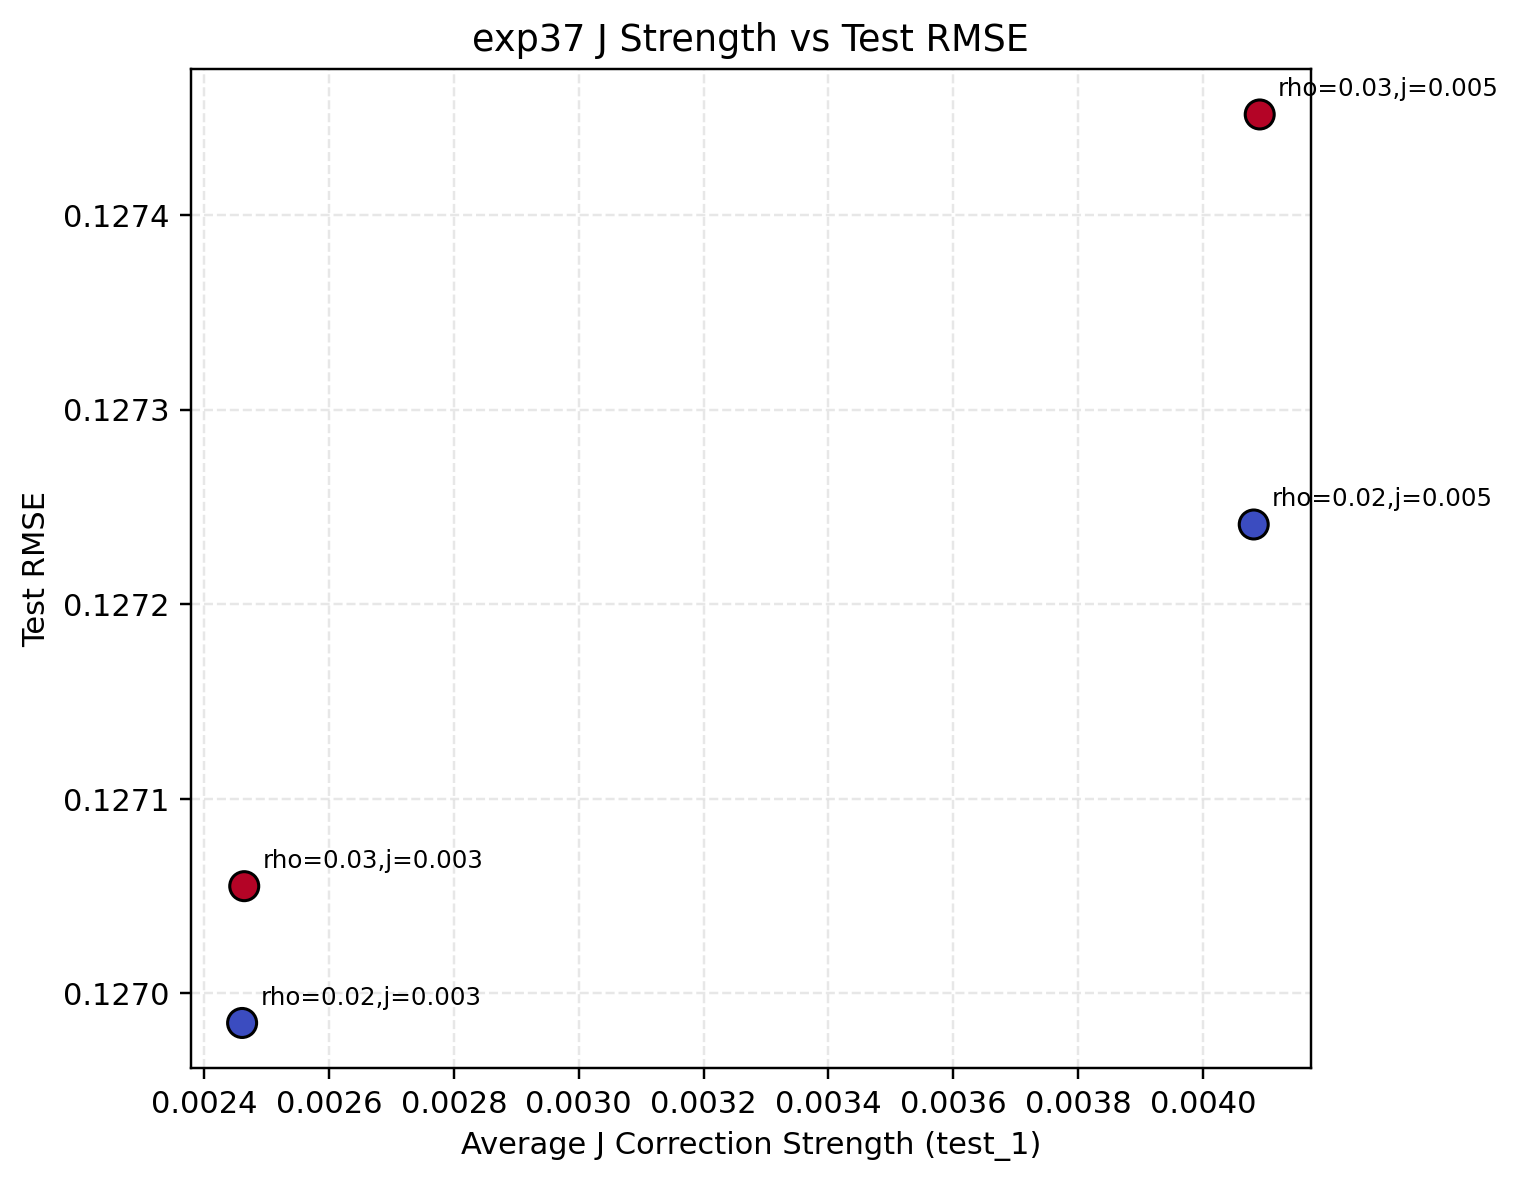
\includegraphics[width=0.92\linewidth]{figures/exp37_j_strength_vs_rmse.png}
\caption{平均 $J$ 修正强度与 test\_1 RMSE 的关系。}
\label{fig:jrmse}
\end{figure}

图 \ref{fig:jrmse} 则直接展示了本文思考过程中的一个关键结论：$J$ 修正并不是越强越好。当前网格中，当平均 $J$ 修正强度约为 $0.00246$ 时，test\_1 RMSE 最低；当其增加到约 $0.00409$ 时，test\_1 RMSE 升至 $0.12745$。这张图非常重要，因为它把“为什么本文坚持弱修正”从经验判断变成了可观察结论。也就是说，弱融合和弱 $J$ 修正不是保守写法，而是由实验行为本身支持的机制选择。

因此，本节对比分析最终支持四点判断。第一，本文方法优于纯经典 fixed，说明量子结构信息在当前受控实验里具有现实价值；第二，本文方法优于 corr 类直接加权，说明结构化信息只有以合适强度接入才有效；第三，本文与物理驱动局部化工作相似之处在于都试图摆脱固定经验局部化，但本文依赖的是量子相似度而不是显式流场特征\cite{sarp2025localization}；第四，本文不同于单纯量子调参或量子退火 DA，因为量子模块本身参与了局地结构建模与更新控制\cite{kotsuki2024qda,felix2024reservoir}。不过，受限于当前结果规模，本节更适合被视为“证据驱动的机制对比”，而不是对所有量子增强同化路线的全面定论。
